\graphicspath{ {imgs/} }
\documentclass[main.tex]{subfiles}
\begin{document}
\chapter{Methods}
The used model is inspired by the network presented in \cite{huang2017lung} and performs with an accuracy of around 80$\%$. The following sections highlight the used methods and give a rough overview about the used tools. A more extensive explanation to them can be found in the appendix.


\section{Software Packages}
The whole programming is done in Python 3.6. 
Use of conda for the environment management 
TensorFlow for the network architecture and computation
Sun Grid Engine of the Institute for the calculations on the grid \ref{appendix:oge}.


\section{Convolutional Neural Network}
In this thesis the main focus was on using a 3d convolutional network. A convolutional neural network is similar to other artificial neural networks (ANNs) in the sense that it only uses forward connections, has an input and output layer and an arbitrary number of hidden layers in between. The hidden layers in a convolutional network are either convolutional or pooling layers. 

Increasing depth to go from detail features like edges to more complex shapes.

Makes sense to use since the structural information like the neighborhood information can be used



The structure of the neural network resembles closely the one described in \cite{huang2017lung}. 



\section{Training}

The input to the network is randomly flipped in x and y plane (examples can be seen in \ref{fig:input}).

\begin{figure}
\begin{center}
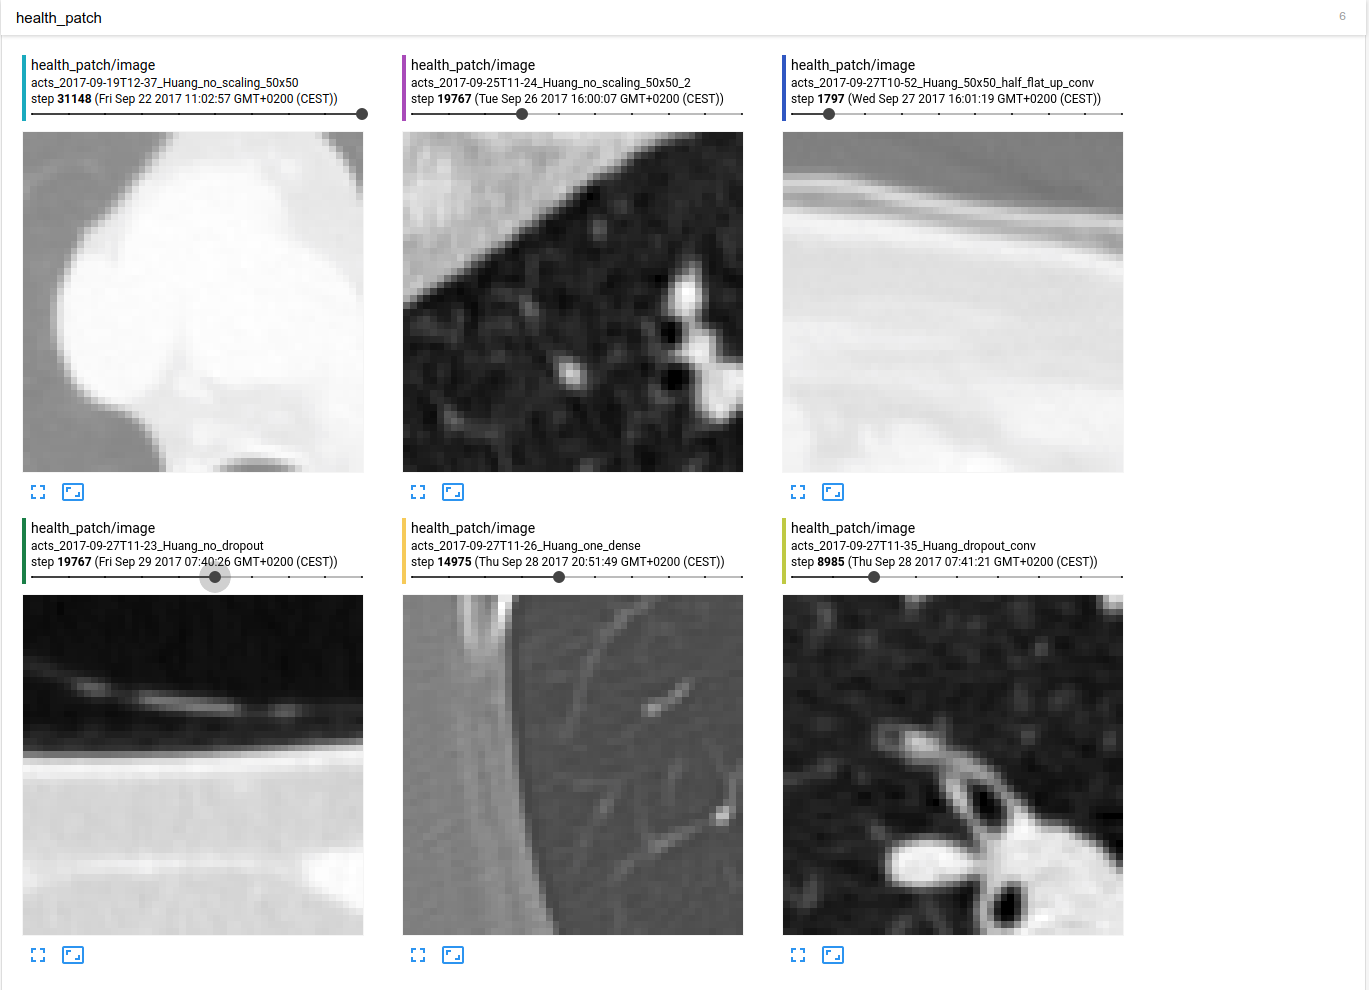
\includegraphics[scale=0.25]{patches-health.png}
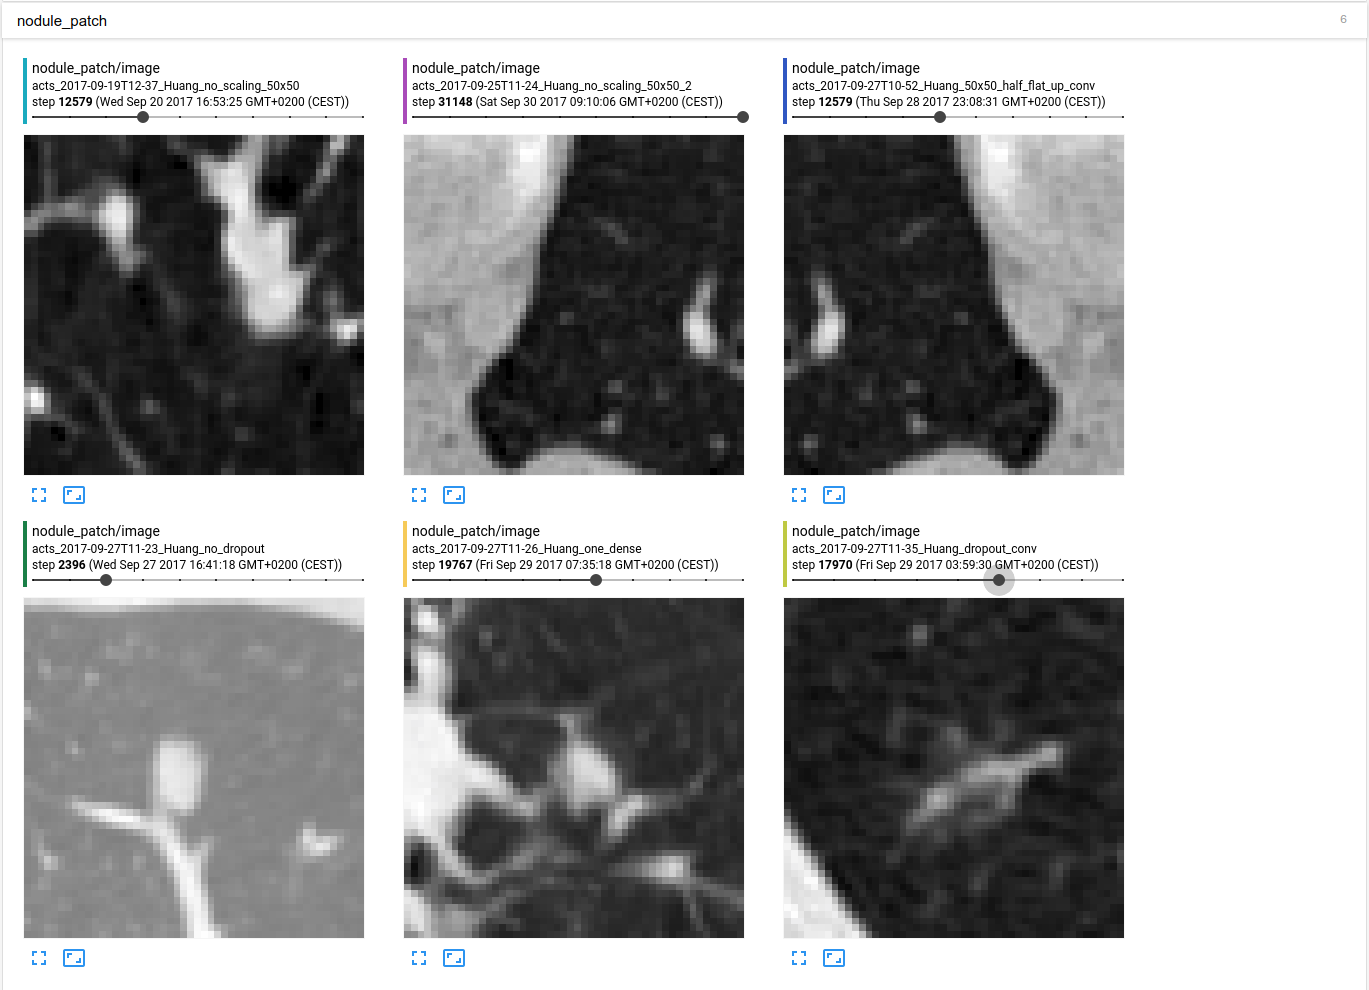
\includegraphics[scale=0.25]{patches-nodule.png}
\end{center}
\caption{Input data for the cases of healthy and nodule patches. The image is taken from Tensorboard and shows in the case of nodules the random permutation of the input data.}
\label{fig:input}
\end{figure}

Why use batchnorm?
Why use dropout?
Compare with and without

\section{Final model}
Show performance of the network and all metrics about number of epochs etc.

\end{document}
